\documentclass[../main.tex]{subfiles}

\begin{document}

\chapter{代码主体结构}
\vspace{-2cm}

在本章节中,我们将对 BasicSR 代码框架进行一个整体介绍,主要包括以下内容:整体框架 (第\ref{code_structure:overview}小节)、配置与注册器 (第\ref{code_structure:register}小节)、数据 (第\ref{code_structure:data}小节)、网络结构 (第\ref{code_structure:arch}小节)、模型 (第\ref{code_structure:model}小节)、损失函数 (第\ref{code_structure:loss}小节)、训练 (第\ref{code_structure:training}小节)、算子 (第\ref{code_structure:ops}小节) 等。通过阅读本章,你将对 BasicSR 有进一步的认识,理解其模块之间的相互关系、以及模块内部的核心工作原理。但我们不对具体函数和代码做具体介绍。如果需要具体函数和代码的介绍,请查阅 BasicSR 的在线 API 文档 (\url{https://basicsr.readthedocs.io/en/latest/})。

\section{整体框架} \label{code_structure:overview}
对于基于深度学习的算法框架,其核心的组成部分包括:\textbf{数据、模型、损失函数、训练}。BasicSR 框架也是大致根据以上部分撰写而成的。下图概括了 BasicSR 的整体组成框架:

\begin{figure}[htbp]
    \begin{center}
        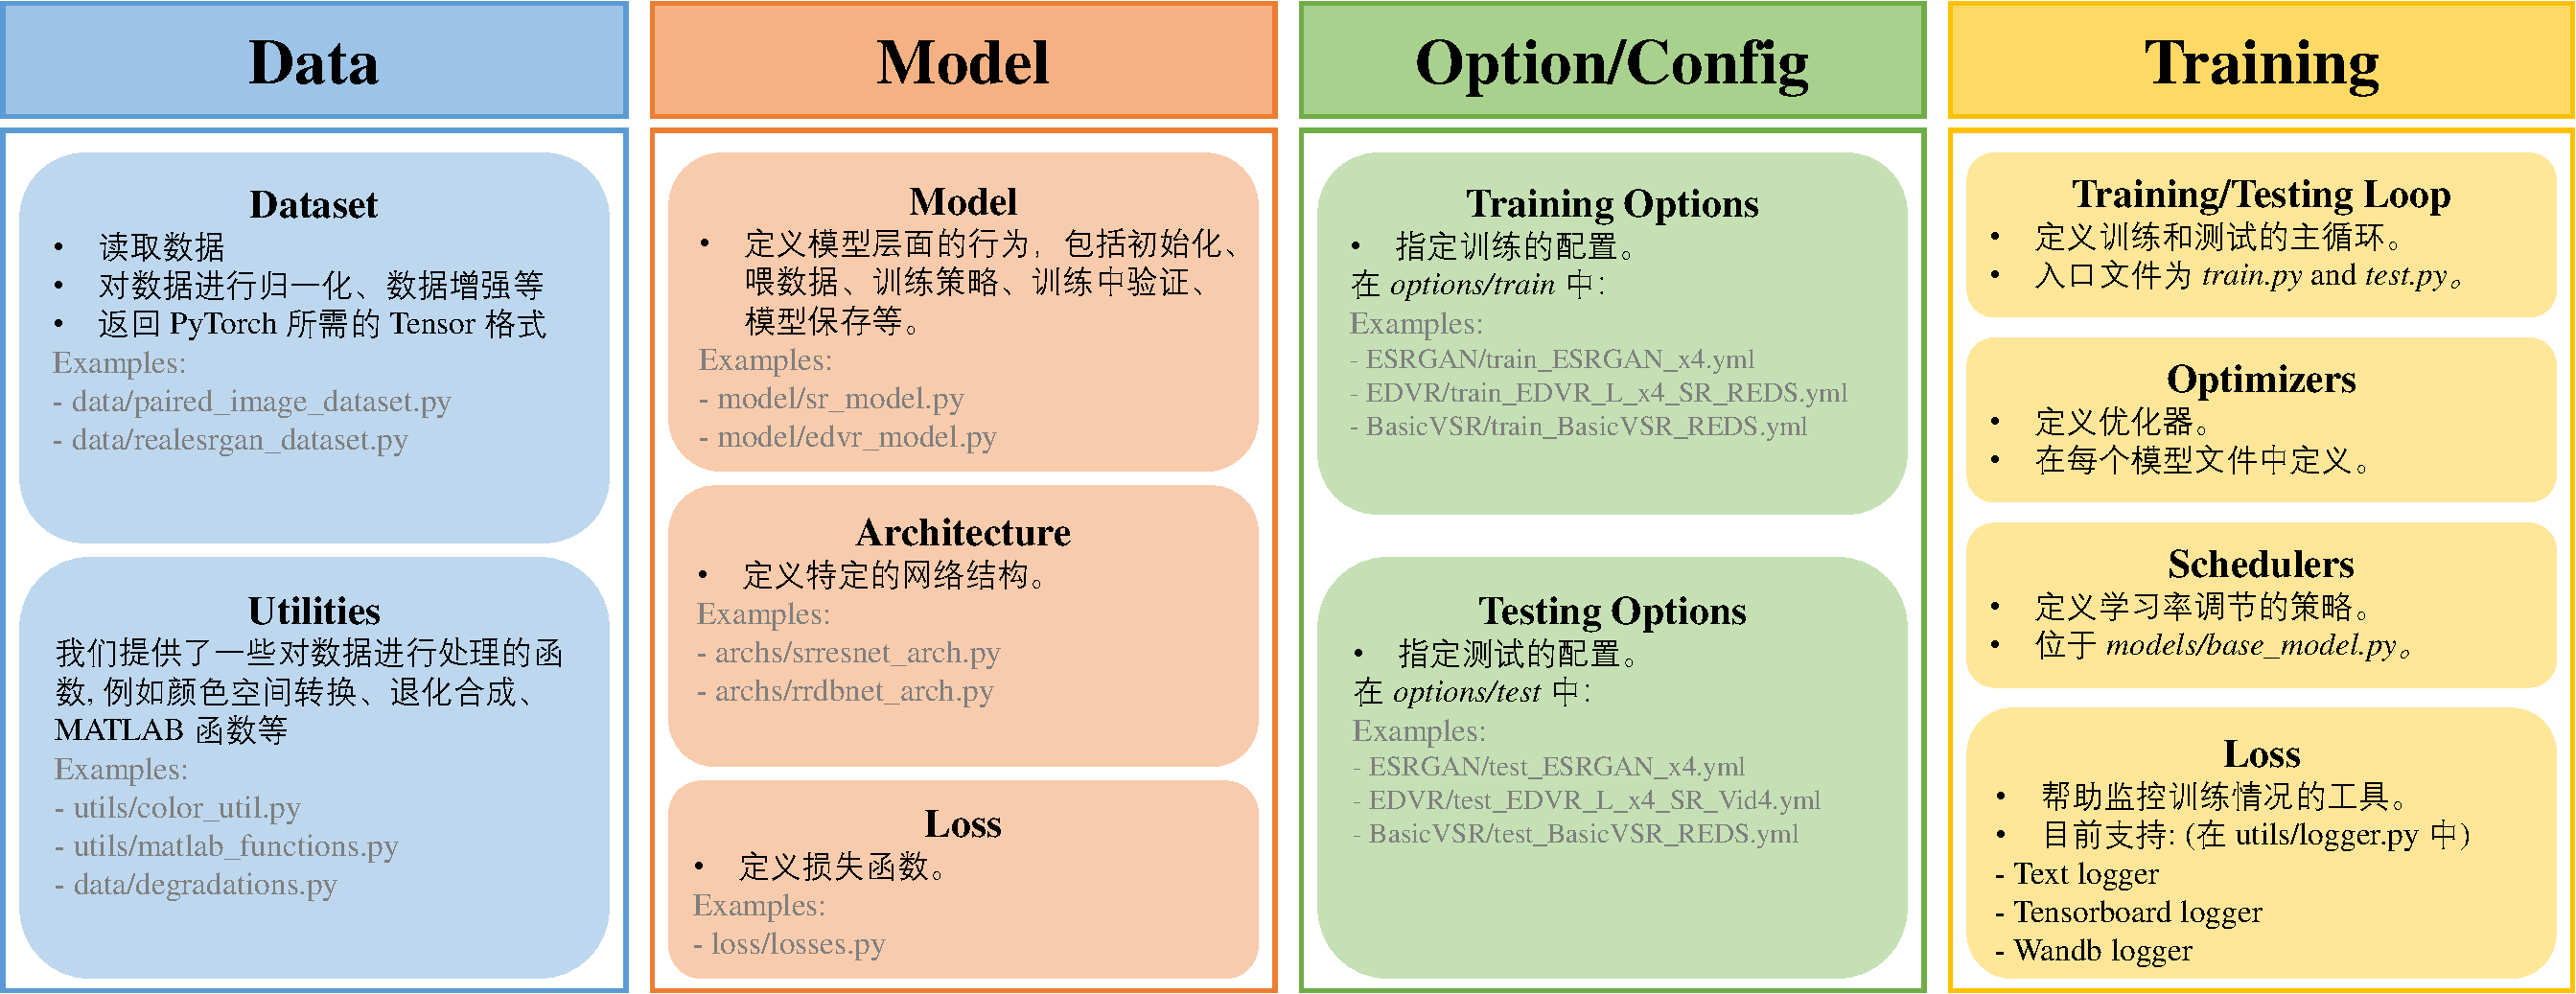
\includegraphics[width=1\linewidth]{figures/main_framework.pdf}
    \end{center}
    \caption{BasicSR 代码整体框架 \todo{把图中 Load data, Apply normalization 这些描述性语言翻译成中文吧。PPT 可以 copy 一页,同时保留中英文的源文件。然后 share 一下 PPT}}
    \label{fig:main_framework}查询。
\end{figure}

\begin{itemize}
    \item 数据 (Data):这个部分主要定义了 Dataset 和 Data Loader 文件, 放在了 \href{https://github.com/XPixelGroup/BasicSR/tree/master/basicsr/data}{data} 目录下。Dataset 用于读取和预处理数据,包括图像读取、归一化 (normalization)、数据增强 (augmentation) 以及封装为 PyTorch Tensor 等。同时,我们也提供了一些辅助函数,帮助使用者自定义自己的数据预处理功能,例如图像色彩空间转换、常用 MATLAB 函数的 Python 版本、常用的图像退化模型 (degradation model) 等。详细说明参见章节\ref{code_structure:data}:\nameref{code_structure:data}。

    \item 模型 (Model):在 \href{https://github.com/XPixelGroup/BasicSR/tree/master/basicsr/models}{models} 目录下,我们提供了常用的模型文件。这些模型文件主要用于定义网络结构与初始化、输入输出数据、一次 forward 的训练过程、保存加载模型等。在 \href{https://github.com/XPixelGroup/BasicSR/tree/master/basicsr/archs}{archs} 目录下,我们提供了常用的网络结构模型文件,包括 SRResNet、ESRGAN、RCAN、SwinIR、EDVR、BasicVSR 等。在 \href{https://github.com/XPixelGroup/BasicSR/tree/master/basicsr/losses}{losses} 文件夹中,我们提供了常用的损失函数,例如 L1/L2 loss、perceptual loss、GAN loss 等。详细说明参见章节\ref{code_structure:arch}:\nameref{code_structure:arch}、章节\ref{code_structure:model}:\nameref{code_structure:model}、章节\ref{code_structure:loss}:\nameref{code_structure:loss}。

    \item 配置 (Option):配置文件放到 \href{https://github.com/XPixelGroup/BasicSR/tree/master/options}{option} 目录下。我们提供了常用模型的训练和测试配置文件。我们使用 \href{https://yaml.org/}{YAML} 来作为配置文件的语言。修改这些 yml 文件可以简易地调整训练过程中的各种超参数。详细说明参见章节\ref{code_structure:register}:\nameref{code_structure:register}。

    \item 训练 (Training):这一部分主要涉及训练的策略和记录训练日志。\href{https://github.com/XPixelGroup/BasicSR/blob/master/basicsr/train.py}{train.py} 和 \href{https://github.com/XPixelGroup/BasicSR/blob/master/basicsr/test.py}{test.py} 是启动模型训练和测试的入口文件,其中定义了训练和测试的 main loop。常见优化器 (optimizer) 的定义可以在 \href{https://github.com/XPixelGroup/BasicSR/blob/master/basicsr/models/base_model.py}{models/base\_model.py} 文件中的 \texttt{get\_optimizer} 函数中找到。学习率的调度策略在 \href{https://github.com/XPixelGroup/BasicSR/blob/master/basicsr/models/base_model.py}{models/base\_model.py}  文件中的 \texttt{setup\_schedulers} 函数中定义。为了方便追踪记录训练的过程,我们提供了相应的 logger 工具,支持直接 print 到屏幕、Tensorboard、Wandb等多种方式,具体代码可以在 \href{https://github.com/XPixelGroup/BasicSR/blob/master/basicsr/utils/logger.py}{utils/logger.py} 中找到。详细说明参见章节\ref{code_structure:training}:\nameref{code_structure:training}。\todo{本章节需要添加 training pipeline、logging 使用方式、test pipeline 的介绍。还有比如 logger 怎么用,validation 放在哪里、怎么用的内容。安排:logging 和 validation 放到 4.5 节 模型里面。training/testing pipeline 放到 4.7 节这里,和入门呼应、互补}

    \item 详细的代码接口文档可以在 \url{http://basicsr.readthedocs.io} 查询。
\end{itemize}

\begin{note} % ---------------- Note block ---------------- %
    \textbf{BasicSR 目录说明}

    你可以在章节\ref{getting_start:content-overview}:\nameref{getting_start:content-overview} 查看到详细的 BasicSR 目录说明。
\end{note}

\section{配置(Options)与注册器(Register)}\label{code_structure:register}
在这一小节,我们先来说配置文件。在 BasicSR 中我们使用 \href{https://yaml.org/}{YAML} 来作为配置文件的语言。

\subsection{配置文件简要说明}
训练的配置文件在 \href{https://github.com/XPixelGroup/BasicSR/tree/master/options/train}{options/train} 中,测试的配置文件在 \href{https://github.com/XPixelGroup/BasicSR/tree/master/options/test}{options/test} 中。通过 option 配置文件,我们可以设置实验名、选择模型、指定 GPU、指定数据路径、选择网络结构、配置训练策略等。

\subsubsection{实验命名}
我们推荐对实验名字进行有意义的命名,方便后续实验以及进行多组实验对比。

我们以 \texttt{001\_MSRResNet\_x4\_f64b16\_DIV2K\_1000k\_B16G1\_wandb} 为例:

\begin{itemize}
\item 001: 我们一般给实验进行数字打头的标号, 方便进行实验管理
\item MSRResNet: 模型名称, 这里指代 Modified SRResNet
\item x4\_f64b16: 重要配置参数, 这里表示放大4倍; 中间feature通道数是64, 使用了16个Residual Block
\item DIV2K: 训练数据集是DIV2K
\item 1000k: 训练了1000k iterations
\item B16G1: Batch size 为16, 使用一卡 GPU 训练
\item wandb: 使用了 wandb, 训练过程上传到了 wandb 云服务器
\end{itemize}

\begin{hl} % ---------------- Highlight block ---------------- %
    \textbf{注意}

    如果在实验名字中有 \texttt{debug} 字样, 则会进入 debug 模式, 即程序会更密集地 log 和 validate, 并且不会使用 tensorboard logger 和 wandb logger。

    具体参见章节\ref{others:debug_mode}:\nameref{others:debug_mode}。
\end{hl}

\subsubsection{配置文件例子说明}

下面,我们以 \href{https://github.com/XPixelGroup/BasicSR/blob/master/options/train/SRResNet_SRGAN/train_MSRResNet_x4.yml}{train\_MSRResNet\_x4.yml} 为例,简单说明配置文件的每个部分。我们先把配置文件贴出来,然后在说明框内详细说明每一个参数的含义。为方便说明,整个配置文件会被分散成不同的块来讲解。

\begin{minted}[xleftmargin=20pt,breaklines,bgcolor=bg]{python}
# Modified SRResNet w/o BN from:
# Photo-Realistic Single Image Super-Resolution Using a Generative Adversarial Network

# ----------- Commands for running
# ----------- Single GPU with auto_resume
# PYTHONPATH="./:${PYTHONPATH}"  CUDA_VISIBLE_DEVICES=0 python basicsr/train.py -opt options/train/SRResNet_SRGAN/train_MSRResNet_x4.yml --auto_resume

# general settings
name: 001_MSRResNet_x4_f64b16_DIV2K_1000k_B16G1_wandb
model_type: SRModel
scale: 4
num_gpu: 1  # set num_gpu: 0 for cpu mode
manual_seed: 0
\end{minted}
\begin{exampleBox}[righthand ratio=0.00, sidebyside, sidebyside align=center, lower separated=false]{一般性配置}

在配置文件的最开始,会有简单的说明,以及默认的运行命令。运行命令的 \texttt{auso\_resume} 表示自动从断点接着训练 (详见章节\ref{others:auto_resume}:\nameref{others:auto_resume})。接下来是一般性配置,主要说明如下:

name:自定义的实验名称。

model\_type:选择模型,如 SRModel,SRGANModel,EDVRModel 等。

scale:超分上采样尺度 (upscale factor)。

num\_gpu:指定使用的 GPU 卡数。\textbf{0 表示 使用CPU,\texttt{auto} 表示自动从可用 GPU 推断}。

manual\_seed:指定随机种子。
\end{exampleBox}

\begin{minted}[xleftmargin=20pt,bgcolor=bg,breaklines]{python}
# dataset and data loader settings
datasets:
  train:
    name: DIV2K
    type: PairedImageDataset
    dataroot_gt: datasets/DF2K/DIV2K_train_HR_sub
    dataroot_lq: datasets/DF2K/DIV2K_train_LR_bicubic_X4_sub
    meta_info_file: basicsr/data/meta_info/meta_info_DIV2K800sub_GT.txt
    # (for lmdb)
    # dataroot_gt: datasets/DIV2K/DIV2K_train_HR_sub.lmdb
    # dataroot_lq: datasets/DIV2K/DIV2K_train_LR_bicubic_X4_sub.lmdb
    filename_tmpl: '{}'
    io_backend:
      type: disk
      # (for lmdb)
      # type: lmdb

    gt_size: 128
    use_hflip: true
    use_rot: true

    # data loader
    use_shuffle: true
    num_worker_per_gpu: 6
    batch_size_per_gpu: 16
    dataset_enlarge_ratio: 100
    prefetch_mode: ~
\end{minted}
\begin{exampleBox}[righthand ratio=0.00, sidebyside, sidebyside align=center, lower separated=false]{数据读取相关配置}
这个部分主要是配置相对应的 dataset 和 data loader 的配置。在这个例子中,这些配置分别用在文件 \href{https://github.com/XPixelGroup/BasicSR/blob/master/basicsr/data/paired_image_dataset.py}{PairedImageDataset} 和 \href{https://github.com/XPixelGroup/BasicSR/blob/master/basicsr/data/__init__.py}{data loader} 中。

datasets 下的 train 表示这是在设置训练数据集和对应的训练 data loader。

name:自定义的数据集名称。

type:读取数据的 Dataset 类,例如 PairedImageDataset 等。详细说明参见章节\ref{code_structure:data}:\nameref{code_structure:data}。

dataroot\_gt:标签 Ground-Truth 图像存放的根目录。

dataroot\_lq:输入 Input 图像存放的根目录。

meta\_info\_file:预先生成的 meta\_info 文件。细节请参看章节\ref{data_preparation:meta_info}:\nameref{data_preparation:meta_info}。\todo{更新链接}

gt\_size:训练阶段,裁剪 (crop) 的 ground-truth 图像的尺寸大小,即训练的 label 大小。

use\_hflip:是否开启水平方向图像增强 (随机水平翻转图像)。

use\_rot:是否开启旋转图像增强 (随机旋转图像)。

use\_shuffle:训练时是否在每一个 epoch 随机打乱数据顺序。

num\_worker\_per\_gpu:每块 GPU 分配的读取数据线程数。

batch\_size\_per\_gpu: 每块 GPU 上的 batch size。

dataset\_enlarge\_ratio: 放大 dataset 的长度倍数 (默认为1)。可以扩大一个 epoch 所需 iterations,详情参见章节\ref{code_structure:data}:\nameref{code_structure:data}。\todo{这块内容需要补足到 数据 这个章节}

prefetch\_mode: 预先读取数据的方式,\textbf{默认为 None,即 $\sim$。\texttt{cpu} 表示使用 CPU prefetcher。\texttt{cuda} 表示使用 CUDA prefetcher。它会多占用一些GPU显存. 注意: 这个模式下, 一定要设置 \texttt{pin\_memory=True}。}详情参见章节\ref{code_structure:data}:\nameref{code_structure:data}。\todo{这块内容需要补足到 数据 这个章节}
\end{exampleBox}

\begin{minted}[xleftmargin=20pt,bgcolor=bg,breaklines]{python}
  val:
    name: Set5
    type: PairedImageDataset
    dataroot_gt: datasets/Set5/GTmod12
    dataroot_lq: datasets/Set5/LRbicx4
    io_backend:
      type: disk

  val_2:
    name: Set14
    type: PairedImageDataset
    dataroot_gt: datasets/Set14/GTmod12
    dataroot_lq: datasets/Set14/LRbicx4
    io_backend:
      type: disk
\end{minted}

\begin{exampleBox}[righthand ratio=0.00, sidebyside, sidebyside align=center, lower separated=false]{validation 配置}

val 部分为训练时 validation 的数据配置。通过定期 validation,我们可以及时观察训练的情况,追踪模型当前的表现。
\end{exampleBox}

    \begin{minted}[xleftmargin=20pt,bgcolor=bg,breaklines]{python}
    # network structures
    network_g:
      type: MSRResNet
      num_in_ch: 3
      num_out_ch: 3
      num_feat: 64
      num_block: 16
      upscale: 4
    \end{minted}
    \begin{exampleBox}[righthand ratio=0.00, sidebyside, sidebyside align=center, lower separated=false]{网络结构相关配置}

    type:选择网络结构模型,例如 MSRResNet,RRDBNet等。

    num\_in\_ch:模型输入的图像通道数。

    numx\_out\_ch: 模型输出的图像通道数。

    num\_feat: 模型内部的 feature map 通道数。

    num\_block: 模型内部基础模块的堆叠数。

    upscale: 上采样倍数。
    \end{exampleBox}
    \begin{minted}[xleftmargin=20pt,bgcolor=bg,breaklines]{python}
    # path
    path:
      pretrain_network_g: ~
      strict_load_g: true
      resume_state: ~
    \end{minted}
    \begin{exampleBox}[righthand ratio=0.00, sidebyside, sidebyside align=center, lower separated=false]{模型存储路径相关配置}

    pretrain\_network\_g: 测试或者 finetune 时,在这里输入保存的模型权重路径。

    strict\_load\_g: 是否严格地根据参数名称一一对应load模型参数。如果选择 false,那么模型对于找不到的参数,会随机初始化;如果选择 true,假如存在不对应的参数,会报错。

    resume\_state: 如训练被打断,可以在这里填写保存的状态文件,恢复训练。
    \end{exampleBox}
    \begin{minted}[xleftmargin=20pt,bgcolor=bg,breaklines]{python}
    # training settings
    train:
      ema_decay: 0.999
      optim_g:
        type: Adam
        lr: !!float 2e-4
        weight_decay: 0
        betas: [0.9, 0.99]

      scheduler:
        type: CosineAnnealingRestartLR
        periods: [250000, 250000, 250000, 250000]
        restart_weights: [1, 1, 1, 1]
        eta_min: !!float 1e-7

      total_iter: 1000000
      warmup_iter: -1  # no warm up

      # losses
      pixel_opt:
        type: L1Loss
        loss_weight: 1.0
        reduction: mean
    \end{minted}
    \begin{exampleBox}[righthand ratio=0.00, sidebyside, sidebyside align=center, lower separated=false]{训练策略相关配置}

    ema\_decay:EMA 参数更新权重。

    optim\_g type: 选择优化器,例如 Adam。

    lr: 初始学习率。

    weight\_decay: 权重衰退参数。

    betas: 优化器动量参数。

    scheduler type: 选择学习率更新策略,例如 CosineAnnealingRestartLR。

    periods: 学习率更新周期。

    restart\_weights: 如果选择学习率 restart 机制,在这里可以指定 restart 时的权重。

    eta\_min: 学习率衰退的最小值。

    total\_iter: 总共进行的训练迭代次数。

    warmup\_iter: warm up 的迭代次数。

    pixel\_opt type: 选择 loss 函数,例如 L1Loss。

    loss\_weight: 指定 loss 的权重。

    reduction: 最终的 loss 取平均或者总和。

    \end{exampleBox}
    \begin{minted}[xleftmargin=20pt,bgcolor=bg,breaklines]{python}
    # validation settings
    val:
      val_freq: !!float 5e3
      save_img: false

      metrics:
        psnr: # metric name, can be arbitrary
          type: calculate_psnr
          crop_border: 4
          test_y_channel: false
          better: higher  # the higher, the better. Default: higher
        niqe:
          type: calculate_niqe
          crop_border: 4
          better: lower  # the lower, the better
    \end{minted}
    \begin{exampleBox}[righthand ratio=0.00, sidebyside, sidebyside align=center, lower separated=false]{validation 相关配置}

    val\_freq: 多少次迭代进行一次 validation。

    save\_img: 是否保存 validation 的图像。

    metrics:validation 时的指标设定。

    type: 选择指标,例如 calculate\_psnr,calculate\_niqe。

    crop\_border: 计算指标时 crop 图像边界像素范围。

    test\_y\_channel: 是否仅在 Y 通道上计算指标。

    better: 该指标是越高越好,还是越低越好。选择 higher 或 者lower,默认为 higher。
    \end{exampleBox}
    \begin{minted}[xleftmargin=20pt,bgcolor=bg,breaklines]{python}
    # logging settings
    logger:
      print_freq: 100
      save_checkpoint_freq: !!float 5e3
      use_tb_logger: true
      wandb:
        project: ~
        resume_id: ~
    \end{minted}
    \begin{exampleBox}[righthand ratio=0.00, sidebyside, sidebyside align=center, lower separated=false]{训练日志相关配置}

    print\_freq: 多少次迭代打印一次训练信息。

    save\_checkpoint\_freq: 多少次迭代保存一次模型权重。

    use\_tb\_logger: 是否开启 Tensorboard。
    \end{exampleBox}

    \subsection{动态实例化与 REGISTER 注册机制}
    \textbf{动态实例化}

    当我们新写了类 (Class) 或函数时,可直接在配置文件中使用。程序会根据配置文件的类名或函数名,自动查找并实例化。这个过程称为动态实例化 (Dynamic Instantiation)。

    具体而言,我们是通过importlib和getattr来实现的。以 data 为例,我们在 \href{https://github.com/XPixelGroup/BasicSR/blob/master/basicsr/data/__init__.py}{data/\_\_init\_\_.py} 中是如下做的:

    1、扫描所有以 \_dataset.py 为结尾的文件 (这是约定);

    2、把这些文件中的类或函数通过 importlib 都 import 进来;

    3、根据配置文件中的名称,通过 getattr 实例化。

    具体操作的代码如下:

    (读者只需知道这个机制即可,以下代码不影响 BasicSR 的直接使用)
    \begin{minted}[xleftmargin=20pt,linenos,bgcolor=bg,breaklines]{python}
    # automatically scan and import dataset modules
    # scan all the files under the data folder with '_dataset' in file names
    data_folder = osp.dirname(osp.abspath(__file__))
    dataset_filenames = [
        osp.splitext(osp.basename(v))[0] for v in scandir(data_folder)
        if v.endswith('_dataset.py')
    ]
    # import all the dataset modules
    _dataset_modules = [
        importlib.import_module(f'basicsr.data.{file_name}')
        for file_name in dataset_filenames
    ]

    ...

    # dynamic instantiation
    for module in _dataset_modules:
        dataset_cls = getattr(module, dataset_type, None)
        if dataset_cls is not None:
            break
    \end{minted}

    我们对以下模块使用了类似的技巧,在使用的时候需要注意文件后缀名称的约定:
    \begin{table}[h]
    \centering
    \begin{tabular}{|c|c|c|}
    \hline
    \textbf{Module} & \textbf{File Suffix} & \textbf{Example} \\ \hline
    Data & \_dataset.py & data/paired\_image\_dataset.py \\ \hline
    Model & \_model.py & basicsr/models/sr\_model.py \\ \hline
    Archs & \_arch.py & basicsr/archs/srresnet\_arch.py \\ \hline
    \end{tabular}
    \caption{动态实例化文件命名约定}
    \end{table}

    \begin{hl} % ---------------- Highlight block ---------------- %
    \textbf{注意}

    1、上面的文件后缀只用在需要的文件中,其他文件命名尽量避免使用以上的后缀。

    2、类名或函数名不能重复。
    \end{hl}

    另外,对 losses 和 metrics,我们也使用了 importlib 和 getattr,但是和上面不一样的是,对于 losses 和 metrics,由于文件数量比较少,改动也少,因此我们不采用扫描文件的方式,而是在新增加类/函数后,需要在相应的 \_\_init\_\_.py 中增加类/函数名称。
    \begin{table}[h]
    \centering
    \begin{tabular}{|c|c|c|}
    \hline
    \textbf{Module} & \textbf{Path} & \textbf{Modify} \\ \hline
    Losses & basicsr/models/losses & basicsr/models/losses/\_\_init\_\_.py \\ \hline
    Metrics & basicsr/metrics & basicsr/metrics/\_\_init\_\_.py \\ \hline
    Archs & \_arch.py & basicsr/archs/srresnet\_arch.py \\ \hline
    \end{tabular}
    \caption{部分类的实例化需要修改对应的 \_\_init\_\_.py 文件}
    \end{table}

    在 log 的时候, loss 项使用 l\_ 开头,这样在 Tensorboard 显示的时候,所有 loss 会被组织到一起。比如在 \href{https://github.com/XPixelGroup/BasicSR/blob/master/basicsr/models/srgan_model.py}{basicsr/models/srgan\_model.py} 中,使用了 l\_g\_pix,l\_g\_percep,l\_g\_gan 等。在 \href{https://github.com/XPixelGroup/BasicSR/blob/master/basicsr/utils/logger.py}{basicsr/utils/logger.py} 中,他们会被组织到一起:
    \begin{minted}[xleftmargin=20pt,bgcolor=bg,breaklines]{python}
    if k.startswith('l_'):
        self.tb_logger.add_scalar(f'losses/{k}', v, current_iter)
    else:
        self.tb_logger.add_scalar(k, v, current_iter)
    \end{minted}

    \textbf{Register 注册机制}

    以上我们介绍了 BasicSR 中的动态实例化机制——代码会根据配置文件指定的Class 名,自动实例化对应的类。这样省去了我们冗余的手动实例化类的操作。

    尽管动态实例化机制很方便,但它仍然存在一些缺陷:1、无法避免重名的问题。一旦出现了类名重名,我们可能无法知道是否实例化了自己想要的类。2、该机制会把文件中所有的类、函数都 import 进来,十分冗余,因为很多类和函数都是中间的量。

    为了解决以上问题,我们进一步引入了 Register 注册机制。我们参考了 FacebookResearch 的 \href{https://github.com/facebookresearch/fvcore}{fvcore} 仓库的函数,定义了 Registry 类。详细代码可查看 \href{https://github.com/XPixelGroup/BasicSR/blob/master/basicsr/utils/registry.py}{basicsr/utils/registry.py}。

    它的主要函数有两个:register() 和 get():
    \begin{minted}[xleftmargin=20pt,linenos,bgcolor=bg,breaklines]{python}
    def register(self, obj=None, suffix=None):
        """
        Register the given object under the the name `obj.__name__`.
        Can be used as either a decorator or not.
        See docstring of this class for usage.
        """
        if obj is None:
            # used as a decorator
            def deco(func_or_class):
                name = func_or_class.__name__
                self._do_register(name, func_or_class, suffix)
                return func_or_class

            return deco

        # used as a function call
        name = obj.__name__
        self._do_register(name, obj, suffix)

    def get(self, name, suffix='basicsr'):
        ret = self._obj_map.get(name)
        if ret is None:
            ret = self._obj_map.get(name + '_' + suffix)
            print(f'Name {name} is not found, use name: {name}_{suffix}!')
        if ret is None:
            raise KeyError(f"No object named '{name}' found in '{self._name}' registry!")
        return ret
    \end{minted}

    它能有效解决上面提到的两个问题:

    1、注册的时候,会强制检查有没有重名,减少了 bug 的产生。

    2、只有在需要时,才会进行注册类或函数,其他中间量不会被注册。

    在 BasicSR 中,我们定义了五个 REGISTER ,相关定义在 \href{https://github.com/XPixelGroup/BasicSR/blob/master/basicsr/utils/registry.py}{basicsr/utils/registry.py} 中:
    \begin{minted}[xleftmargin=20pt,linenos,bgcolor=bg,breaklines]{python}
    DATASET_REGISTRY = Registry('dataset')
    ARCH_REGISTRY = Registry('arch')
    MODEL_REGISTRY = Registry('model')
    LOSS_REGISTRY = Registry('loss')
    METRIC_REGISTRY = Registry('metric')
    \end{minted}

    需要注册的时候,我们使用了 Python 装饰器,即在类/函数前面加上下面的语句:
    \begin{minted}[xleftmargin=20pt,linenos,bgcolor=bg,breaklines]{python}
    from basicsr.utils.registry import ARCH_REGISTRY
    from .arch_util import default_init_weights, make_layer, pixel_unshuffle

    @ARCH_REGISTRY.register()
    class RRDBNet(nn.Module):
        def __init__(self):
            super(RRDBNet, self).__init__()
            ......
    \end{minted}

    于是,上面的 RRDBNet 网络结构就被注册上啦。

    其他的 DATASET,ARCH,MODEL,LOSS 都是类似的操作。它们都是注册了类,实例化的时候根据配置的 Class name 进行实例化。

    注意,METRIC 稍微有点特殊,它是注册了函数,一样的用法,但是会根据函数名来调用相对应的函数。后面介绍 METRIC 的时候,再具体展开。

    值得注意的是,即使我们使用了 REGISTER 机制,import 问题还是存在,即 Python 怎么知道你写了某个网络结构文件。

    为了尽量少修改文件,我们沿用了动态实例化时候的做法,约定网络结构的文件使用  \_arch.py 结尾,然后自动扫描,import 进来。

    其他的几个注册器的约定:

    1、DATASET\_REGISTRY:以 \_dataset.py 结尾

    2、ARCH\_REGISTRY:以 \_arch.py 结尾

    3、MODEL\_REGISTRY:以 \_model.py 结尾

    4、LOSS\_REGISTRY:以 \_loss.py 结尾 (目前只有一个文件,所以还没有添加相应的扫描的代码,后面会添加上)

    5、METRIC\_REGISTRY: 这个因为改动很少,我们就保留了 在\_\_init\_\_.py 文件中 import 的方式:
    \begin{minted}[xleftmargin=20pt,linenos,bgcolor=bg,breaklines]{python}
    from copy import deepcopy

    from basicsr.utils.registry import METRIC_REGISTRY
    from .niqe import calculate_niqe
    from .psnr_ssim import calculate_psnr, calculate_ssim

    __all__ = ['calculate_psnr', 'calculate_ssim', 'calculate_niqe']


    def calculate_metric(data, opt):
        """Calculate metric from data and options.
        Args:
            opt (dict): Configuration. It must contain:
                type (str): Model type.
        """
        opt = deepcopy(opt)
        metric_type = opt.pop('type')
        metric = METRIC_REGISTRY.get(metric_type)(**data, **opt)
        return metric
    \end{minted}

    总结一下,当我们在新开发网络结构的时候,只要做两件事,修改两个文件就好了。BasicSR 背后的动态实例化和 REGISTRY 机制会帮你完成剩下的事。

    1、写一个单独的网络结构文件 (以 \_arch.py 结尾)。在写好的 Class 前加上 @ARCH\_REGISTRY.register() 装饰器。

    2、在配置文件中指定使用哪一个网络结构,即上面的 Class name。




\section{数据 (Data Loader)}\label{code_structure:data}
    数据是机器学习的动力来源。这一章节我们介绍 BasicSR 的数据读取和处理机制。在 \href{https://github.com/XPixelGroup/BasicSR/tree/master/basicsr/data}{basicsr/data/} 目录下,我们提供了常用的 Dataset 文件。

    \dirtree{%
        .1 ROOT\_DIR.
        .2 BasicSR.
        .3 basicsr.
        .4 data.
        .5 \_\_init\_\_.py.
        .5 paired\_image\_dataset.py.
        .5 single\_image\_dataset.py.
        .5 realesrgan\_paired\_dataset.py.
        .5 realesrgan\_dataset.py.
        .5 reds\_dataset.py.
        .5 vimeo90k\_dataset.py.
        .5 video\_test\_dataset.py.
        .5 ffhq\_dataset.py.
        .5 data\_util.py.\DTcomment{提供了数据读取相关的函数}.
        .5 data\_sampler.py.
        .5 degradations.py.\DTcomment{提供若干图像退化的合成函数}.
        .5 prefetch\_dataloader.py.
        .5 transforms.py.\DTcomment{提供了常用的数据增强函数}.
    }

    BasicSR 提供的常用数据集的 Dataset 文件如下:

    \begin{table}[h]
    \centering
    \resizebox{\textwidth}{26mm}{
    \begin{tabular}{|c|c|c|c|}
    \hline
    \textbf{类} & \textbf{任务} & \textbf{训练/测试} & \textbf{描述} \\ \hline
    PairedImageDataset & 图像超分 & 训练 & 读取成对的训练数据 \\ \hline
    SingleImageDataset & 图像超分 & 测试 & 只读取 low quality 的图像, 用于没有 GT 的测试中 \\ \hline
    REDSDataset & 视频超分 & 训练 & 读取 REDS 的训练数据集 \\ \hline
    Vimeo90KDataset & 视频超分 & 训练 & 读取 Vimeo90K 的训练数据集 \\ \hline
    VideoTestDataset & 视频超分 & 测试 & 基础的视频超分测试集, 支持 Vid4,  REDS 测试集 \\ \hline
    VideoTestVimeo90KDataset & 视频超分 & 测试 & 继承 VideoTestDataset;Vimeo90K 的测试数据集 \\ \hline
    VideoTestDUFDataset & 视频超分 & 测试 & 继承 VideoTestDataset; DUF算法的测试数据集, 支持 Vid4 \\ \hline
    FFHQDataset & 人脸生成 & 训练 & 读取 FFHQ 的训练数据集 \\ \hline
    \end{tabular}
    }
    \caption{BasicSR 提供的数据处理类}
    \end{table}

    下面,我们以 PairedImageDataset 为例,大致讲解 Dataset 文件的内容。
    \begin{minted}[xleftmargin=20pt,linenos,breaklines,bgcolor=bg,breaklines]{python}
    @DATASET_REGISTRY.register()
    class PairedImageDataset(data.Dataset):
        def __init__(self, opt):
            super(PairedImageDataset, self).__init__()
            self.opt = opt
            # file client (io backend)
            self.file_client = None
            self.io_backend_opt = opt['io_backend']
            self.mean = opt['mean'] if 'mean' in opt else None
            self.std = opt['std'] if 'std' in opt else None
    \end{minted}

    在 option 文件中可以指定数据读取方式 (opt['io\_backend'])。

    我们支持三种读取数据的模式:

    1、直接从 lmdb 格式的文件中读取;

    2、若提供了 meta\_info 文件,则直接从该文件中列出的文件路径读取数据;

    3、输入文件目录,代码会自动扫描该目录中的文件,然后读取。


    \begin{minted}[xleftmargin=20pt,linenos,breaklines,bgcolor=bg]{python}
            self.gt_folder, self.lq_folder = opt['dataroot_gt'], opt['dataroot_lq']
            if 'filename_tmpl' in opt:
                self.filename_tmpl = opt['filename_tmpl']
            else:
                self.filename_tmpl = '{}'

            if self.io_backend_opt['type'] == 'lmdb':
                self.io_backend_opt['db_paths'] = [self.lq_folder, self.gt_folder]
                self.io_backend_opt['client_keys'] = ['lq', 'gt']
                self.paths = paired_paths_from_lmdb([self.lq_folder, self.gt_folder], ['lq', 'gt'])
            elif 'meta_info_file' in self.opt and self.opt['meta_info_file'] is not None:
                self.paths = paired_paths_from_meta_info_file([self.lq_folder, self.gt_folder], ['lq', 'gt'], self.opt['meta_info_file'], self.filename_tmpl)
            else:
                self.paths = paired_paths_from_folder([self.lq_folder, self.gt_folder], ['lq', 'gt'], self.filename_tmpl)
    \end{minted}

    从 option 文件中读取 GT 图像目录 (opt['dataroot\_gt']) 和输入图像目录 (opt['dataroot\_lq'])。

    根据指定的文件读取方式,选择相应的读取函数。

    1、lmdb 方式, 选择 paired\_paths\_from\_lmdb 函数;

    2、meta\_info\_file 方式,选择 paired\_paths\_from\_meta\_info\_file 函数;

    3、一般的文件目录方式,选择 paired\_paths\_from\_folder 函数。

    \begin{minted}[xleftmargin=20pt,linenos,breaklines,bgcolor=bg]{python}
        def __getitem__(self, index):
            if self.file_client is None:
                self.file_client = FileClient(self.io_backend_opt.pop('type'), **self.io_backend_opt)

            scale = self.opt['scale']

            # Load gt and lq images. Dimension order: HWC; channel order: BGR;
            # image range: [0, 1], float32.
            gt_path = self.paths[index]['gt_path']
            img_bytes = self.file_client.get(gt_path, 'gt')
            img_gt = imfrombytes(img_bytes, float32=True)
            lq_path = self.paths[index]['lq_path']
            img_bytes = self.file_client.get(lq_path, 'lq')
            img_lq = imfrombytes(img_bytes, float32=True)
    \end{minted}

    \_\_getitem\_\_() 函数是 Dataset 中最关键的函数,定义了每一次迭代时数据是如何读取并处理的。 图像通过 FileClient 读取后,shape 为 HWC, 其中颜色通道的排列顺序为 BGR。图像此时为 [0, 1] 的 float32 格式。

    \begin{minted}[xleftmargin=20pt,linenos,breaklines,bgcolor=bg]{python}
            # augmentation for training
            if self.opt['phase'] == 'train':
                gt_size = self.opt['gt_size']
                # random crop
                img_gt, img_lq = paired_random_crop(img_gt, img_lq, gt_size, scale, gt_path)
                # flip, rotation
                img_gt, img_lq = augment([img_gt, img_lq], self.opt['use_hflip'], self.opt['use_rot'])

            # color space transform
            if 'color' in self.opt and self.opt['color'] == 'y':
                img_gt = rgb2ycbcr(img_gt, y_only=True)[..., None]
                img_lq = rgb2ycbcr(img_lq, y_only=True)[..., None]
    \end{minted}

    这一部分首先对读取的图像进行 crop 处理 (从原图中随机 crop 出一个 patch),然后进行随机的水平翻转和旋转,进行数据增强。如果要使用单通道训练 (YCbCR 颜色空间中的 Y 通道),代码会对 GT 和 input 进行颜色转换。

    \begin{minted}[xleftmargin=20pt,linenos,breaklines,bgcolor=bg]{python}
            # crop the unmatched GT images during validation or testing, especially for SR benchmark datasets
            if self.opt['phase'] != 'train':
                img_gt = img_gt[0:img_lq.shape[0] * scale, 0:img_lq.shape[1] * scale, :]

            # BGR to RGB, HWC to CHW, numpy to tensor
            img_gt, img_lq = img2tensor([img_gt, img_lq], bgr2rgb=True, float32=True)
            # normalize
            if self.mean is not None or self.std is not None:
                normalize(img_lq, self.mean, self.std, inplace=True)
                normalize(img_gt, self.mean, self.std, inplace=True)

            return {'lq': img_lq, 'gt': img_gt, 'lq_path': lq_path, 'gt_path': gt_path}
    \end{minted}

    在测试时,由于上下采样的原因,有时候模型的输出和原始的图像大小会出现不匹配的情况。例如,原始图像大小为 $530 \times 530$,在 $\times 4$  超分中,原图会下采样变成 $132 \times 132$ 的输入,模型会超分后会得到 $528 \times 528$ 的输出,与原图大小不匹配,进而无法直接计算 PSNR 等指标。于是,为了避免这个问题,我们在测试时,会 crop 原始图像多余的像素,使其分辨率和模型输出相同。

    另外,我们对图像格式进行一些转换:把 BGR 格式转换为 RGB;把 HWC 的排列,转换为 Pytorch所需的 CHW。如果指定了数据集的均值 (mean) 和标准差 (std),我们将会进一步对数据进行Z-score标准化操作。

    最后,我们返回一个字典,包括输入的 LQ 图像,作为标签的 GT 图像,以及他们的路径。


\section{网络结构 (Architecture)} \label{code_structure:arch}
    在 \href{https://github.com/XPixelGroup/BasicSR/tree/master/basicsr/archs}{basicsr/archs/} 目录下,我们提供了若干经典的网络结构。

    \begin{table}[h]
    \centering
    {
    \begin{tabular}{|c|c|c|c|}
    \hline
    \textbf{网络结构} & \textbf{任务} & \textbf{文件} & \textbf{描述} \\ \hline
    EDSR & 图像超分 & edsr\_arch.py & 论文EDSR结构 \\ \hline
    SRResNet & 图像超分 & srresnet\_arch.py & 论文SRGAN的Generator \\ \hline
    RRDB & 图像超分 & rrdbnet\_arch.py & 论文ESRGAN的Generator \\ \hline
    RCAN & 图像超分 & rcan\_arch.py & 论文RCAN的结构 \\ \hline
    SwinIR & 图像超分 & swinir\_arch.py & 论文SwinIR的结构 \\ \hline
    ECBSR & 图像超分 & ecbsr\_arch.py & 论文ECBSR的结构 \\ \hline
    SRVGG & 图像超分 & srvgg\_arch.py & VGG结构改造的SR网络 \\ \hline
    EDVR & 视频超分 & edvr\_arch.py & 论文EDVR的结构 \\ \hline
    BasicVSR & 视频超分 & basicvsr\_arch.py &  论文BasicVSR的结构\\ \hline
    BasicVSR++ & 视频超分 & basicvsrpp\_arch.py &  论文BasicVSR++的结构\\ \hline
    DUF & 视频超分 & duf\_arch.py &  论文DUF的结构\\ \hline
    TOF & 视频超分 & tof\_arch.py &  论文TOF的结构\\ \hline
    HiFaceGAN & 人脸生成 & hifacegan\_arch.py &  论文HiFaceGAN的结构\\ \hline
    DFDNet & 人脸生成 & dfdnet\_arch.py &  论文Deep Face Dictionary Network的结构\\ \hline
    StyleGAN2  & 人脸生成 & stylegan2\_arch.py &  论文StyleGAN2的结构 \\ \hline
    RIDNet  & 图像去噪 & ridnet\_arch\_arch.py &  论文RIDNet的结构 \\ \hline
    VGG  & 工具结构 & vgg\_arch.py &  经典VGG结构 \\ \hline
    InceptionV3  & 工具结构 & inception.py &  经典InceptionV3的结构,用于计算FID指标 \\ \hline
    VGG \& UNet  & 工具结构 & discriminator\_arch.py &  在GAN训练中,常用的Discriminator结构 \\ \hline
    SpyNet  & 工具结构 & spynet\_arch.py &  论文SpyNet的结构 \\ \hline
    \end{tabular}
    }
    \caption{BasicSR 提供的经典网络结构}
    \end{table}



\section{模型 (Model)}\label{code_structure:model}

- Base模型

- 其他模型

- 继承关系

\section{损失函数 (Loss)}\label{code_structure:loss}

\section{训练(优化器与学习率调度器)}\label{code_structure:training}

\section{算子}\label{code_structure:ops}

\end{document}